%%%%%%%%%%%%%%%%%%%%%%%%%%%%%%%%%%%%%%%%%%%%%%%%%%%%%%%%%%%%%%%%%%%%%%%%%%%%%%
%
% タイトル TeX用テンプレート 
% バージョン 2014-11-8 (Sat) 初版
% 作成者 Kouhei Ito
% 作成場所 野々市市中林 DeuxMKK
% 用途 2段組レポートの作成等
%
%%%%%%%%%%%%%%%%%%%%%%%%%%%%%%%%%%%%%%%%%%%%%%%%%%%%%%%%%%%%%%%%%%%%%%%%%%%%%%%%
%\documentclass[11pt,twocolumn]{jsarticle}
\documentclass[11pt]{si2016}
\usepackage[dvipdfmx]{graphicx}
\usepackage{amsmath,amssymb}
\usepackage{url}
\usepackage{nidanfloat}

%% 体裁

% ページレイアウト(A4:297 mm × 210 mm,1 インチ = 25.4 mm)
% http://www.biwako.shiga-u.ac.jp/sensei/kumazawa/tex/layout.html
% http://www.slis.tsukuba.ac.jp/~fujisawa.makoto.fu/cgi-bin/wiki/index.php?TeX%A5%E1%A5%E2#p61e1b46
% 上 20 mm,下 22 mm,左右 20 mm の余白設定
\setlength{\topmargin}{-20truemm}
\setlength{\headheight}{10truemm}
\setlength{\headsep}{4.6truemm}
\setlength{\textheight}{255truemm}
\setlength{\oddsidemargin}{-5.4truemm}
\setlength{\evensidemargin}{-5.4truemm}  % twoside オプション指定時のみ有効
\setlength{\textwidth}{170truemm}
% \setlength{\columnsep}{8truemm}
\setlength{\columnsep}{6truemm}


%%%%%%%%%%%%%%%%%%%%%%%%%%%%%%%%%%%%%%%%%%%%%%%%%%%%%%%%%%%%%%%%%%%%%%%%%%%%%%%%
\title{音声認識による接客ロボットの開発}
\author{金沢工業高等専門学校 澤田茂人}
\date{2016-09-07}
%%%%%%%%%%%%%%%%%%%%%%%%%%%%%%%%%%%%%%%%%%%%%%%%%%%%%%%%%%%%%%%%%%%%%%%%%%%%%%%%
\begin{document}
\maketitle
\begin{abstract}
音声認識について今から解説する.音声認識とはコンピューターを用いて音声を入力し入力した音声を文字にして示すことである.
\end{abstract}


\tableofcontents
%%%%%%%%%%%%%%%%%%%%%%%%%%%%%%%%%%%%%%%%%%%%%%%%%%%%%%%%%%%%%%%%%%%%%%%%%%%%%%%%
\section{はじめに}
\subsection{研究の背景}
今回の音声認識は食堂にて注文を取るロボットがある場合,人件費の経費削減ができるため制作してほしいという要望があった.そこで音声でのやりとりをするためのシステムを究明する必要があると考え,本研究を開始した.食堂で注文を取るロボットに使用した音声を認識させるシステムについて今から述べていく.


\subsection{研究の目的}
食堂にてPCを実装したロボットに音声認識をするためJulius,Open-JTalk,認識すべき単語,マイクを準備し実際に店で禁煙か喫煙かの判断や「あちらの席へどうぞ」「こちらの席へどうぞ」のようなレベルの案内をすることを目的とする.図\ref{fig:yousu}に音声認識をしようとしたときのイメージ図を示す.


\begin{figure*}[h]
 \begin{center}
  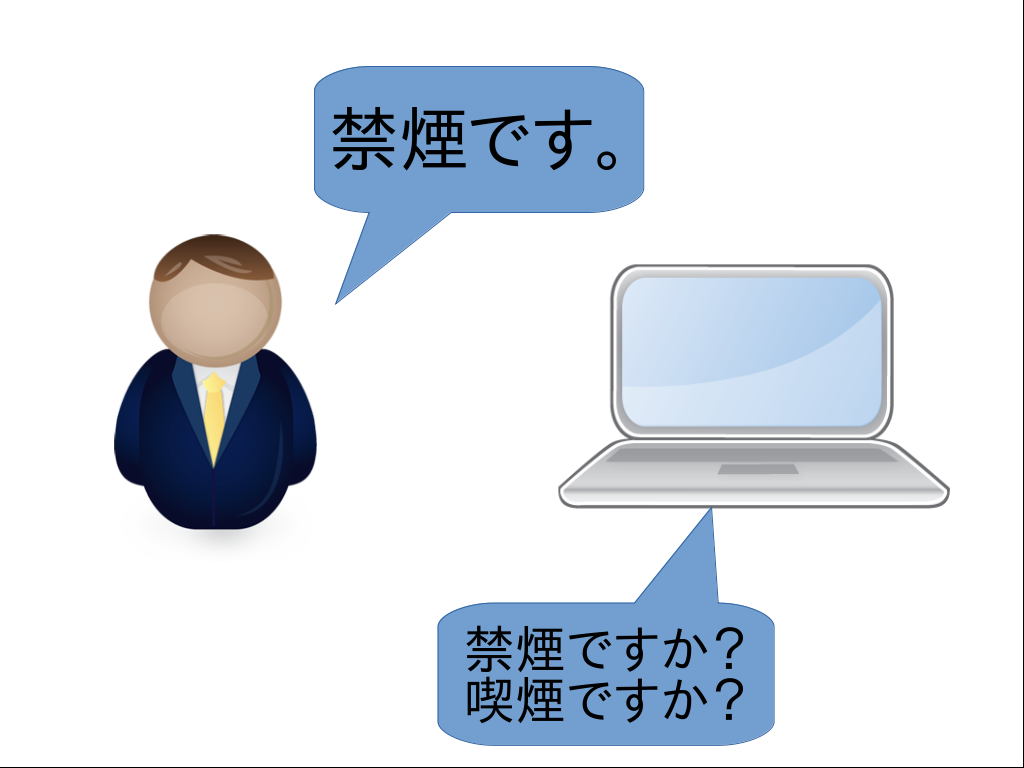
\includegraphics[width=35mm]{img/sukusho.png}
  \caption{様子}
  \label{fig:yousu}
 \end{center}
\end{figure*}


\section{飲食店での接客について}
\subsection{接客の仕事内容}
お客さまから注文を取り,出来上がった料理や飲み物を運び,空いた皿の片付け,レジ業務を行うのが主な仕事である.本研究のために協力していただいた店でははじめに「いらっしゃいませ」と客をお出迎えする.
「何名様ですか」と人数の確認をし,このときに禁煙か喫煙かの確認も行う.5人以上の客でなおかつ禁煙の場合は「ただいま席をお作りしますので少しお待ちください」と言う.
水とメニューを置く.メニューを置くときに水が出せない場合はメニューのみ出す.黒板メニューと呼ばれるものがある場合はお知らせする.小学生の低学年以下の子供がいる場合はキッズプレートを勧める.また,水を出すときは「いらっしゃいませ」と言いながらお客様の前に置き小さな子供がいるときはグラスが手の届かないように親の前などに置く.客の荷物などでテーブルが塞がている場合は端にまとめて置く.
オーダーを取るとき「お決まりですか?」と声を掛ける.決まっていない場合でも早めに聞くことで聞き忘れやオーダーの機器遅れによる客の不満も未然に防ぐ事ができるので必ず行う.注文するものが決まっている場合は客の見ているページをよく見て確認しながら伝票へ記入する.聞き取りにくかった場合や客が勘違いしていそうな場合は「こちらの〜でよろしいですか?」や「こちらの〜ですが」などメニューを手差ししながら説明や確認をしてミスを防ぐ.注文するものが決まってない場合は「ではお決まりになったらお呼びください.」と言う.
そしてドリンクバーやパン,ライスの確認を行う.
オーダーの確認を行うときは「オムライスセットがおひとつ,ステーキライスがおひとつでよろしいですか?」のように復唱して確認を行う.このとき,客の顔をみて確認を行う.ドリンクバー付の場合は「あちらからご自由にお取り下さい」と場所を説明しながら確認する.
厨房にオーダーを出す場合は大きな声で「お願いします.ランチ・ワン.パスタセットスリーです.」と言う.伝票下一枚を伝票版につけて厨房に渡す.残り一枚はホールコーナーに貼る.
シルバーセットを使用する場合は「失礼します」と言い,昼の場合はBセット以外のシルバーをかごに入れて客の前に持って行き,夜の場合は人数分のかごにおしぼりを入れて客の前に持って行く.
料理を出すときは「お待たせしました,オムライスです.」と言いながら出す.出す場所がわからない場合は「お待たせしました,オムライスのお客様は?」と確認をし,置く.料理出しの帰りは他のテーブルに目を配る.食事の終わってる所から「お下げしてよろしいですか?」と声掛けして食器を下げる.
伝票チェック時に料理が出る都度ホールコーナーにある伝票にチェックを入れる.出揃ったら客のテーブルの下の伝票を伏せて置いてくる.デザートがある場合は下の伝票をデザートコーナーに持って行き上の伝票はホールコーナの下段に下ろす.デザートがある場合は食後の進み具合に気を配り食事が終わったらデザートコーナーに「1番にアフターお願いします」とオーダーする.
客に呼ばれた場合,席まで早足で行き「はい,お呼びですか.」とお伺いする.追加オーダーの場合オーダーを下の伝票に記入・復唱確認後,食べ終わっている客の食器を下げてくる.
食後にデザートが付くメニューの場,空いた食器をさげる時に遅くなったときの不安を防ぐために「デザートをお持ちします.」と声を掛ける.
レジではまず「ありがとうございます」といい,「オムライスおひとつで80円です.」「1000円お預かりします.」「140円のお返しです.」の流れでお金のやりとりを行う.また,複数の場合は「日替わりがおひとつとオムライスがおひとつで1720円です.」「5000円お預かりします.」「3000円と280円のお返しです.」「ありがとうございました.」と言う.レジで会計をする際に別払いと思われる客の場合は「ご一緒でよろしいですか?」と確認する.
カットはお客様がいる場合お冷サービスをしながら「お下げします.」と声を掛けて下げる.帰られた後は重ねて下げる.


\subsection{研究として検討する仕事}
前述では接客の仕事内容を挙げたが今回,接客をするロボットを制作するにあたり,店の入口付近で客がタバコを吸うかどうかの判断や「あちらの席へどうぞ」「こちらの席へどうぞ」の案内をすることが研究として検討する仕事となる.


\subsection{今年度のロボット}
今年度のロボットは図\ref{fig:robot}に示すロボットを使用して音声認識を行う.


\begin{figure*}[h]
 \begin{center}
  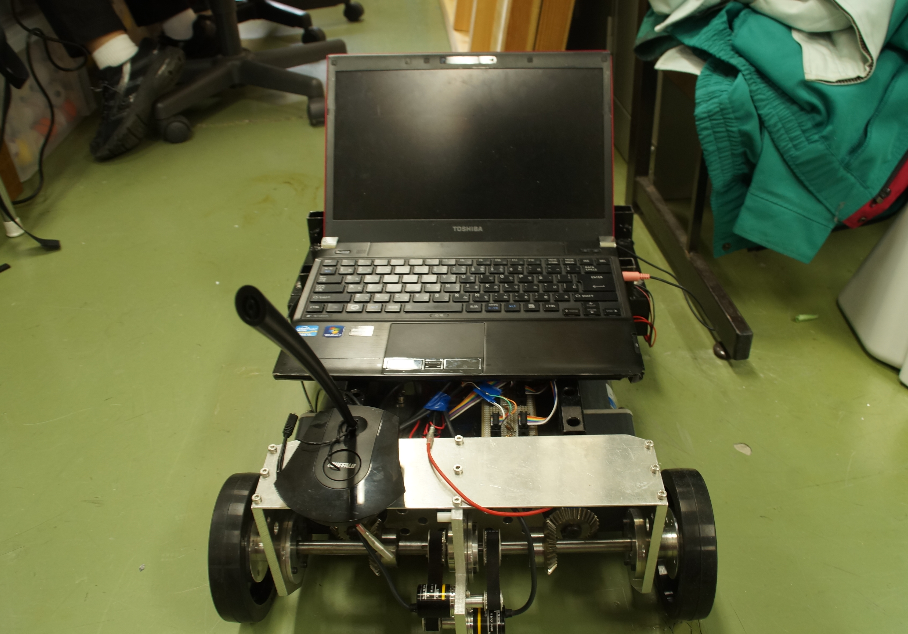
\includegraphics[width=40mm]{img/robo.png}
  \caption{使用したロボット}
  \label{fig:robot}
 \end{center}
\end{figure*}


\section{Julius}
Juliusは,音声認識システムの開発・研究のためのオープンソースの高性能な汎用大語彙連続音声認識エンジンである.数万語彙の連続音声認識を一般のPC上でほぼ実時間で実行できる.また,高い汎用性を持ち,発音辞書や言語モデル・音響モデルなどの音声認識の各モジュールを組み替えることで,様々な幅広い用途に応用できる.[1]Juliusはコマンド1つで起動させることができ,オプションでサーバモードや予め録音しておいた音声を認識させるなど元から用意したプログラムの改良せずに済むため今回は音声をマイクから認識させ,オプションでテキストファイルに変換するために使用する.


\section{Open-JTalk}
Open-JTalkは,日本語テキストを音声に変換するシステムである.ここではc言語を用いてaplayコマンドをsystem関数によりJuliusより得たテキストファイルの内容を音声として発するために使用する.


\section{TCP/IP}
今回、Juliusを使用するにあたり,サーバーモードとして使用することでPC1台の中のみで操作を行う事ができ,サーバとクライアントをTCP/IP経由で繋ぐためにC言語を用いてコンパイルし,繋ぐことができるように改良した.


\section{研究手順}
(1)食堂にて入口前にPCを実装したロボットを設置する.


(2)客が入ったことを認識したら「いらっしゃいませ」と音声を発する.


(3)「いらっしゃいませ」と発した直後に「おタバコお吸いになりますか?」と発する.


(4)「禁煙です」「吸わないです」「吸いません」と答えたとき,「あちらの席になります」と答える.


(5)「喫煙です」「吸います」と答えたとき,「こちらの席になります」と答える.


\section{研究結果}
Juliusで音声を入力し,認識することを確認した.そのときの様子を図\ref{fig:ninshiki}に示す.また,Juliusをサーバモードとして動かした.この時の様子を図\ref{fig:sa-ba-1}に示す.サーバモードで動かす際に研究用にc言語で作成したクライアントをjuliusとつなぎ,音声を認識させた.しかし文字化けが起こった.そのときの様子を図\ref{fig:moji}に示す.Open-Jtalkでは研究用としてc言語でプログラムを組み,必要な音声を出力することに成功した.そのときの様子を図\ref{fig:konpairu}に示す.


\begin{figure*}[h]
 \begin{center}
  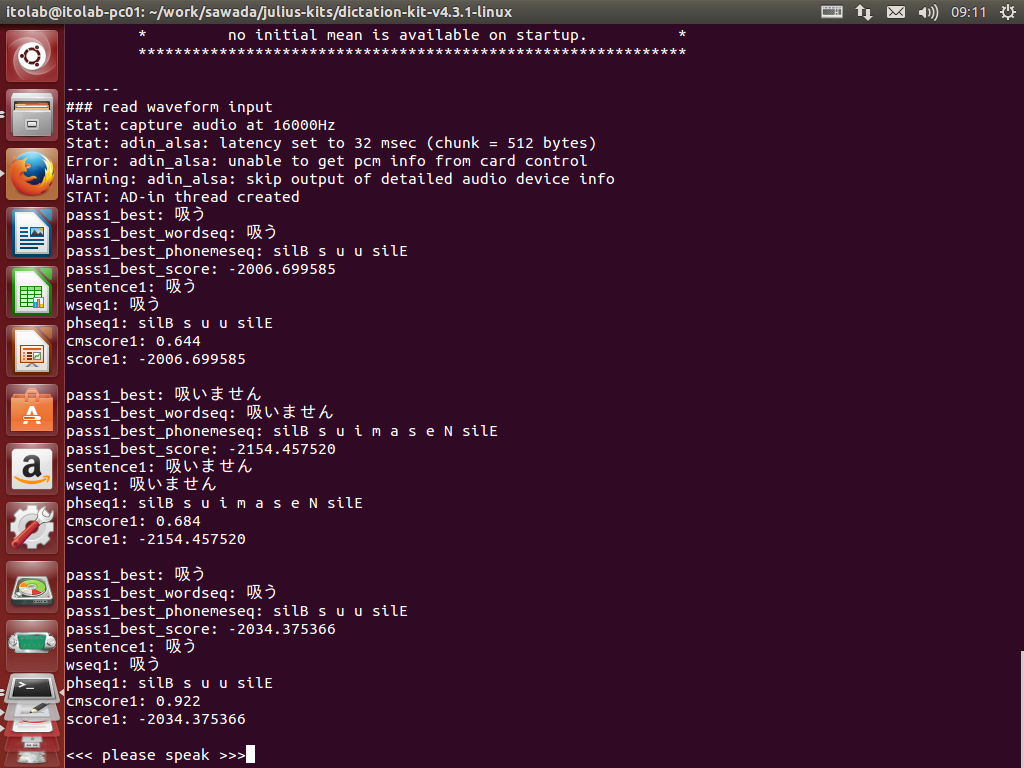
\includegraphics[width=35mm]{img/ninshiki.png}
  \caption{認識結果}
  \label{fig:ninshiki}
 \end{center}
\end{figure*}


\begin{figure*}[h]
 \begin{center}
  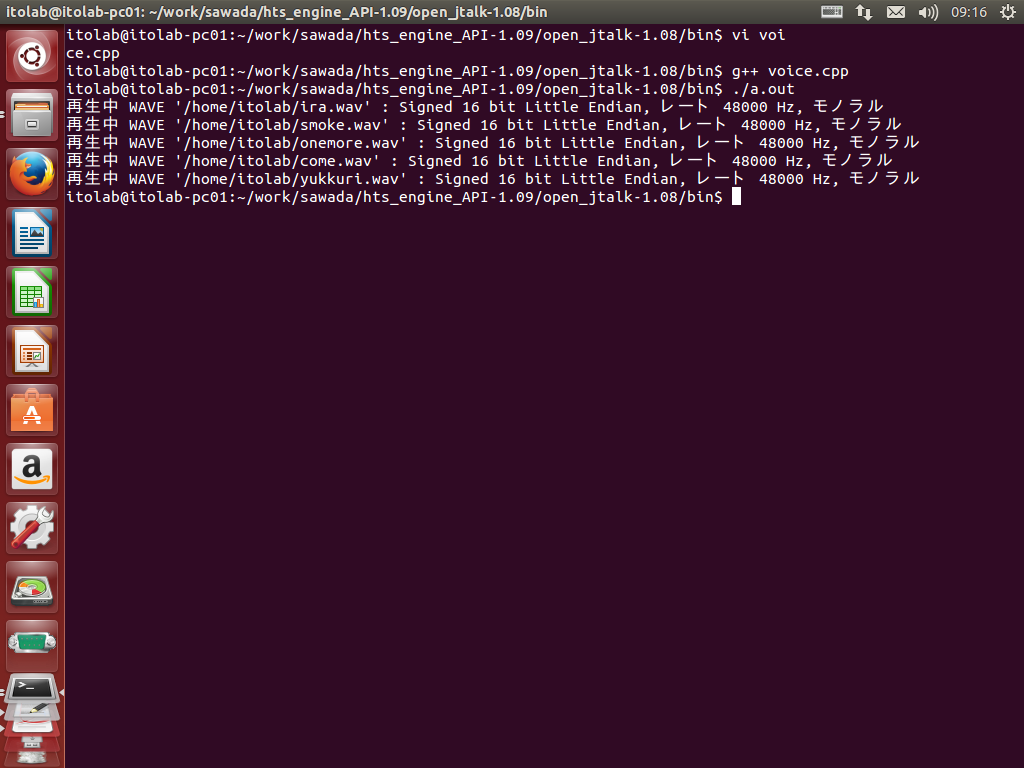
\includegraphics[width=35mm]{img/konpairu.png}
  \caption{音声の出力}
  \label{fig:konpairu}
 \end{center}
\end{figure*}


\begin{figure*}[h]
 \begin{center}
  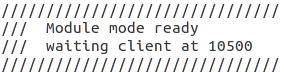
\includegraphics[width=35mm]{img/sa-ba1.png}
  \caption{サーバモード}
  \label{fig:sa-ba-1}
 \end{center}
\end{figure*}


\begin{figure*}[h]
 \begin{center}
  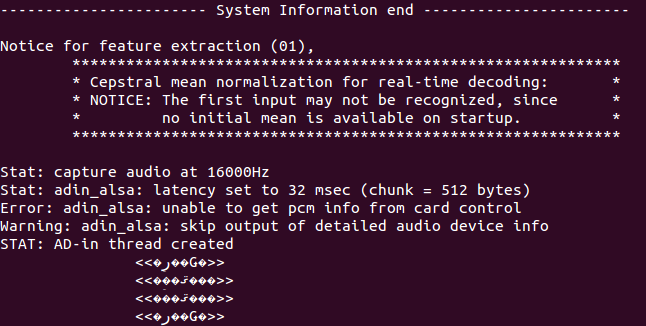
\includegraphics[width=35mm]{img/moji.png}
  \caption{文字化け}
  \label{fig:moji}
 \end{center}
\end{figure*}


\section{考察}
今回はJuliusを使用して音声の入力やOpen-JTalkを使用して音声の出力を行うことができたがそれぞれ独立して操作を行ったため,Juliusを使用する際にテキストファイルを出力させ,そのテキストファイルをOpen-JTalkが音声として出力させるためのツールを見つけて使用することができれば実際に食堂にて使用することができると考えられる.


\section{おわりに}
今回ロボットに音声認識をさせることで人件費の削減につなげられるのではないかと考え,JuliusやOpen-JTalkで音声の入出力を行うことと決めJuliusでの音声の認識やOpen-JTalkでの音声の出力に成功した.今後はJuliusとOpen-JTalkを連携する手段を見つけ,人間とロボットの対話を行えるようにする.


\begin{thebibliography}{1}
  \bibitem{キー1} 第7章 言語モデル・https://julius.osdn.jp/juliusbook/ja/desc_lm.html・2016/09/02閲覧


  \bibitem{キー2} Raspberry PiでJuliusを使った音声認識(外部連携編)・http://hyottokoaloha.hatenablog.com/entry/2015/07/03/131305・2016/09/02閲覧


  \bibitem{キー3} mkdfa.pl リファレンス・マニュアル・https://julius.osdn.jp/juliusbook/ja/mkdfa_pl.html・2016/09/09閲覧


\appendix
\section{今回使用したもの}
yomiファイルとは認識させるために準備した単語を書き込んだものである.今回使用したyomiファイルを図\ref{fig:yomi}に示す.vocaファイルとはカテゴリごとに単語の表記と読み(音素列)を登録する[1].今回使用したvocaファイルを図\ref{fig:voca}に示す.grammarファイルとは構文制約を単語のカテゴリを終端規則として記述したファイルである.[1]今回使用したgrammarファイルを図\ref{fig:grammar}に示す.dfaファイルとはオートマトン定義ファイルであり,grammarで記述される文法制約を有限個の状態と状態遷移のある振る舞いの抽象的なモデルに変換したものである.[1]今回使用したdfaファイルを図\ref{fig:dfa}に示す.termファイルとは単語カテゴリ番号と実際のカテゴリ名の対応をさせるために用いるファイルである[2].今回使用したtermファイルを図\ref{fig:term}に示す.dicファイルとは単語を認識させるための辞書ファイルである.後述のdictファイルとの相違点はjconfファイルに指定する単語を認識させるためである.今回使用したdicファイルを図\ref{fig:dic}に示す.dictファイルとは単語を認識させるための辞書ファイルである.[3]dicファイルとの相違点はdfaファイルと連動させる点にある.今回使用したdictファイルを図\ref{fig:dict}に示す.


\begin{figure*}[h]
 \begin{center}
  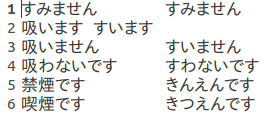
\includegraphics[width=35mm]{img/yomi.png}
  \caption{yomiファイル}
  \label{fig:yomi}
 \end{center}
\end{figure*}


\begin{figure*}[h]
 \begin{center}
  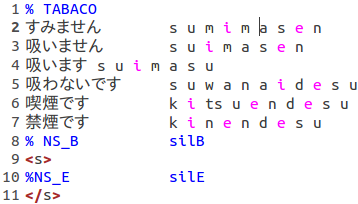
\includegraphics[width=35mm]{img/voca.png}
  \caption{vocaファイル}
  \label{fig:voca}
 \end{center}
\end{figure*}


\begin{figure*}[h]
 \begin{center}
  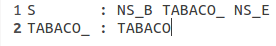
\includegraphics[width=35mm]{img/grammar.png}
  \caption{grammarファイル}
  \label{fig:grammar}
 \end{center}
\end{figure*}


\begin{figure*}[h]
 \begin{center}
  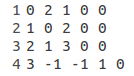
\includegraphics[width=35mm]{img/dfa.png}
  \caption{dfaファイル}
  \label{fig:dfa}
 \end{center}
\end{figure*}


\begin{figure*}[h]
 \begin{center}
  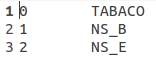
\includegraphics[width=35mm]{img/term.png}
  \caption{termファイル}
  \label{fig:term}
 \end{center}
\end{figure*}


\begin{figure*}[h]
 \begin{center}
  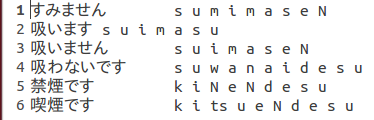
\includegraphics[width=35mm]{img/dic.png}
  \caption{dicファイル}
  \label{fig:dic}
 \end{center}
\end{figure*}


\begin{figure*}[h]
 \begin{center}
  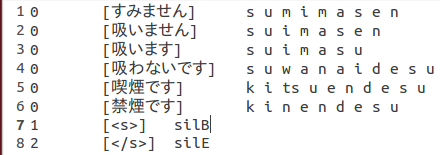
\includegraphics[width=35mm]{img/dict.png}
  \caption{dictファイル}
  \label{fig:dict}
 \end{center}
\end{figure*}



\end{thebibliography}
%%%%%%%%%%%%%%%%%%%%%%%%%%%%%%%%%%%%%%%%%%%%%%%%%%%%%%%%%%%%%%%%%%%%%%%%%%%%%%%%%


\end{document}
